% !TeX root = ../paper_observer_consciousness.tex

Ein Gehirnprozess in dem quantenmechanische Superpositionen denkbar sind
die Aktivität von Neuronen, den Grundbausteinen der Informationsverarbeitung im 
Gehirn. Das komplexe Netzwerk aus $\sim \num{e11}$ Neuronen kann auch durch
Forschungsergebnisse anderer Wissenschaften mit dem Bewusstsein in Zusammenhang
gebracht werden. 

Eine schematische Darstellung einer Nervenzelle ist in \cref{fig:neuron} gezeigt.
Auf das, für diese Betrachtung, Notwendigste reduziert stellen Neuronen im Prinzip
ein System mit zwei möglichen Zuständen dar, die feuern (aktiv) und 
nicht-feuern (passiv) genannt werden. Der Zustand ist dabei von der Konzentration
von Na$^{+}$-Ionen im Inneren der Nervenzelle abhängig, bei hohen Konzentrationen
feuert die Nervenzelle bei niedrigen nicht. Eine Superposition zwischen einer 
feuernden und nicht-feuernden Nervenzelle lässt sich demnach vereinfacht als räumliche 
Superposition von Na$^{+}$-Ionen annehmen. Die räumliche Trennung dieser beiden Orte 
ist dabei von der Größenordnung der Zellwände $h \sim \SI{10}{\nano\meter}$.

Um nun Aussagen über die Dekohärenz-Zeitskalen machen zu können muss zunächst 
die Anzahl der Ionen bestimmt werden, die sich gleichzeitig in Superposition befinden.
Diese Anzahl wird über eine einfache Abschätzung der Ladungsverteilung in der Nervenzelle
ermittelt. Im feuernden Zustand beträgt die Potentialdifferenz zwischen dem Inneren und Äußeren
der Zelle $U_1 \sim \SI{0.03}{\volt}$ während diese im nicht-feuernden Zustand $U_0 \sim \SI{-0.07}{\volt}$
beträgt. Die Anzahl $N$ der Na$^{+}$-Ionen ergibt sich damit und realistischen Abschätzungen\footnote{$h=\SI{8}{nm}$, $d=\SI{10}{\micro\metre}$, $L=\SI{10}{\centi\metre}$, $f=\num{e-3}$} für 
die Ausmaße einer Nervenzelle zu 
\begin{empheq}{equation}
		N = \frac{\pi dLf\epsilon_{0}}{qh}\del{U_{1} - U_{0}} \approx \num{e6}.
\end{empheq}

\begin{figure}
	\centering
	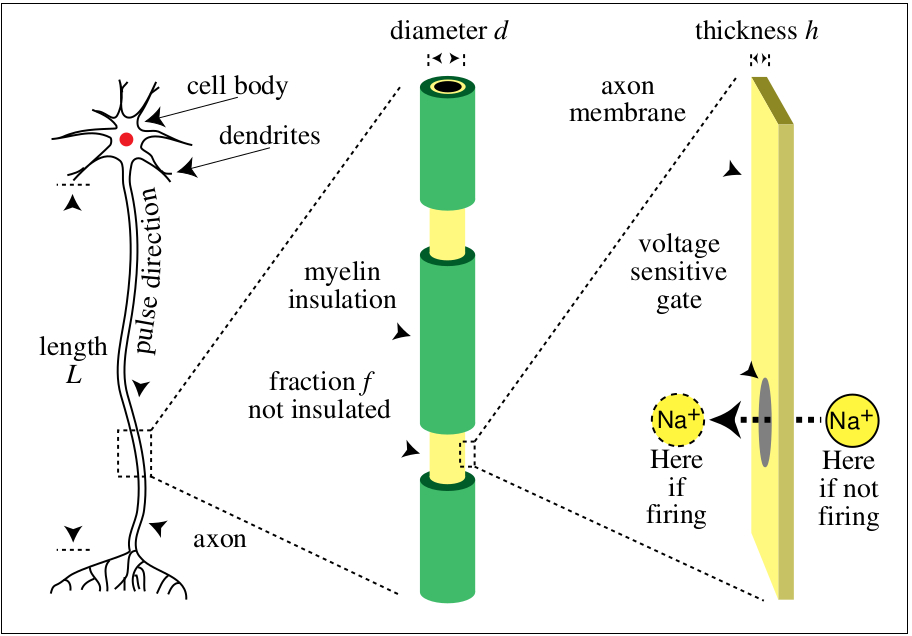
\includegraphics[scale=0.4]{graphics/neuron_schematic.jpg}
	\caption{Schematische Darstellung einer Nervenzelle. Hervorgehoben sind die Größen, die für die Abschätzung der 
		Anzahl der Na$^{+}$-Ionen verwendet werden, die sich in Superposition befinden.\cite{Tegmark_99} \label{fig:neuron}}
\end{figure}

Für die Abschätzung der Größenordnung der Dekohärenz-Zeitskala werden die drei am häufigsten auftretenden
Wechselwirkungen mit der Umgebung
betrachte. Dies sind zum einen Stöße der Na-Ionen mit anderen Ionen oder Wassermolekülen und zum anderen
Coulomb-Abstoßung zwischen den gleich geladenen Na-Ionen.
Die Zeitentwicklung des Zustandes $\rho$ lässt sich für diese drei Wechselwirkungen allgemein mit  
\begin{empheq}{align}
	\label{eq:time_evolution}
	\rho(r, r^{\prime},t_{0}+t) = \rho(r, r^{\prime},t_{0}) f(r,r^{\prime},t)
\end{empheq}
beschreiben wobei die Funktion $f(r,r^{\prime},t)$ von der Wechselwirkung 
und nicht von dem Zustand des Ions abhängt. Eine detailliert Betrachtung der Berechnungen
ist in \cite{Tegmark_99} zu finden. 
Als Dekohärenz-Zeitskalen für die drei betrachteten Wechselwirkungen ergeben sich die in 
\cref{tab:decoherence_time} dargestellten.
\begin{table}
	\centering
	\begin{tabular}{lc}
		\toprule
		Wechselwirkung & $\tau_{dec}$\\
		\midrule
		Stoß mit Ion & \SI{e-20}{s} \\ 
		Stoß mit H$_2$O & \SI{e-20}{s} \\ 
		Coulombabstoßung & \SI{e-19}{s} \\ 
		\bottomrule
	\end{tabular}
	\caption{Zeitskalen der Dekohärenz aufgrund der betrachteten Wechselwirkungen der Na$^{+}$-Ionen
		in Superposition. Abgewandelt aus: \cite{Tegmark_99} \label{tab:decoherence_time}}
\end{table}

Es zeigt sich als das Superpositionen von Neuronen, wie sie hier betrachtet wurde auf Zeitskalen der 
Größenordnung \SI{e-20}{s} zerstört werden. Verglichen mit den typischen Dynamik-Zeitskalen, die für 
die schnellsten Neuronen bei etwa \SI{e-3}{s} liegen, zeigt sich ein Unterschied von etwa 17 Größenordnungen.
Entsprechend kann gefolgert werden das Superpositionen zwischen unterschiedlichen Neuronenzuständen bereits 
bei der Entstehung unterdrückt werden und diese Gehirnprozesse somit klassisch beschrieben werden müssen. 
 